% This is my HW 6 solution set.

\documentclass[12pt, leqno]{article}
\usepackage{amsfonts, amsmath, amssymb}
\usepackage{fancyhdr}
\usepackage{hyperref}
\usepackage{graphicx}
\newcounter{qcounter}
\usepackage[lofdepth,lotdepth]{subfig}
\usepackage[maxfloats=40]{morefloats}
\usepackage{float}
\usepackage{}
\usepackage[english]{babel}
\usepackage{tabularx}
\providecommand{\abs}[1]{\lvert#1\rvert} % absolute value
\providecommand{\normd}{\mathcal{N}} % normal distribution
\providecommand{\norm}[1]{\lVert#1\rVert} % norm
\newcommand{\macheps}{\epsilon_{\mbox{\scriptsize mach}}}
\usepackage[ampersand]{easylist}
\makeatletter
\newcommand{\distas}[1]{\mathbin{\overset{#1}{\kern\z@\sim}}}%
\newsavebox{\mybox}\newsavebox{\mysim}
\newcommand{\distras}[1]{%
  \savebox{\mybox}{\hbox{\kern3pt$\scriptstyle#1$\kern3pt}}%
  \savebox{\mysim}{\hbox{$\sim$}}%
  \mathbin{\overset{#1}{\kern\z@\resizebox{\wd\mybox}{\ht\mysim}{$\sim$}}}%
}
\makeatother

\begin{document}
\pagestyle{fancy}
\lhead{Syed Rahman}
\rhead{STA6866}

\begin{center}
{\large {\bf Homework 5}} \\
\end{center}
\paragraph{1.} We use $JAGS$ to run a Gibbs Samper to estimate the
joint density of $(\mu,\sigma)$ and $(\psi_j)_{j=1}^{12}$. We use a thin of
2, a burn-in of 100000 and collect 1 million samples. 

The probability that the odds ratio is greater than 1
can be estimated using:
\[
\hat{P}(e^{{\psi}_1} >1) = \frac{1}{n}{\sum_{i=1}^n
  I{[e^{\psi^{(i)}_1}>1]}} =  0.98796
\]
Figure \ref{density} shows a plot for the posterior density of the
odds ratio using a kernel density estimator, while Figure \ref{acf}
displays the autocorrelation and Figure \ref{trace} shows the trace for
$e^{{\psi}_1}$.

\begin{figure}
\begin{center}
  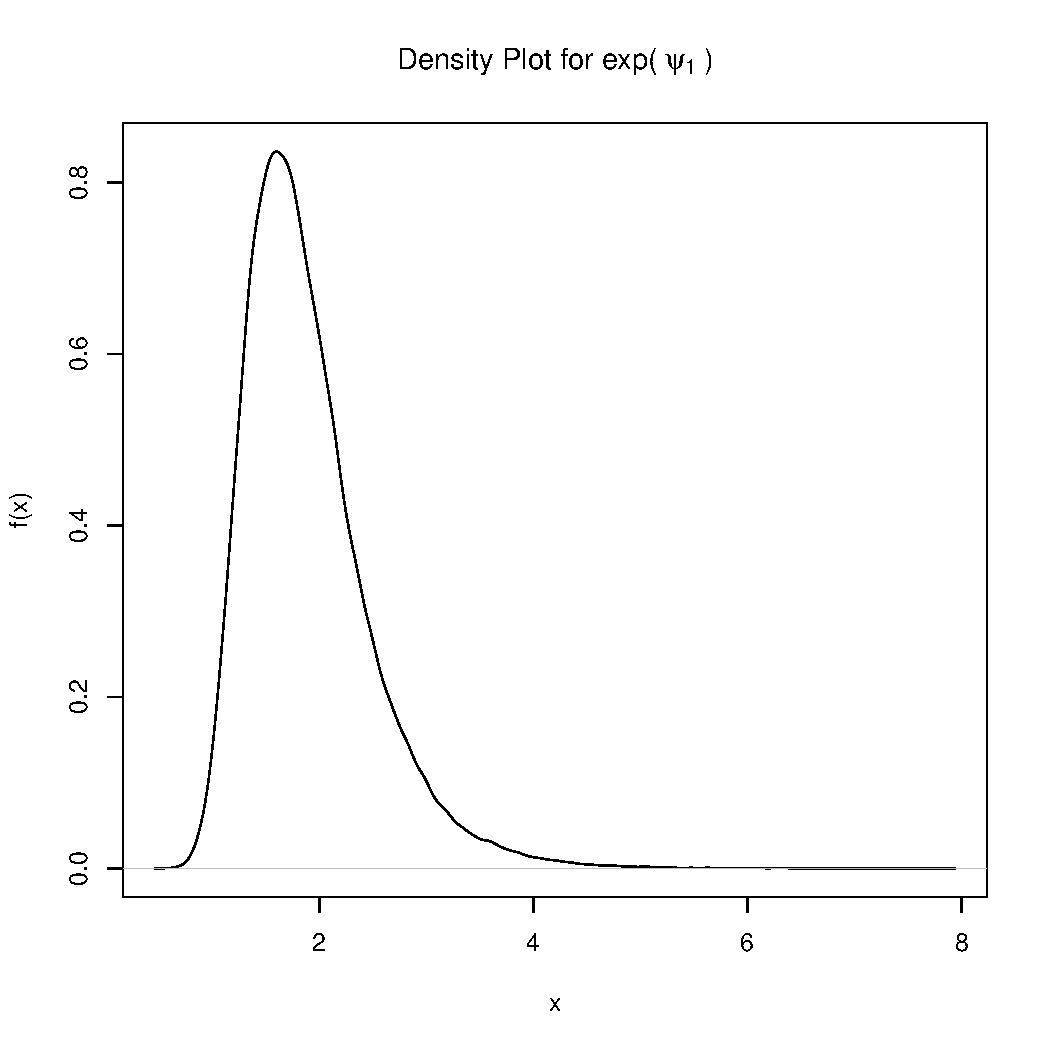
\includegraphics[scale=0.55]{psi1density.pdf}
\end{center}
\caption{Density plot for odds ratio} 
\label{density}
\end{figure} 

\begin{figure}
\centering
\subfloat[]
  {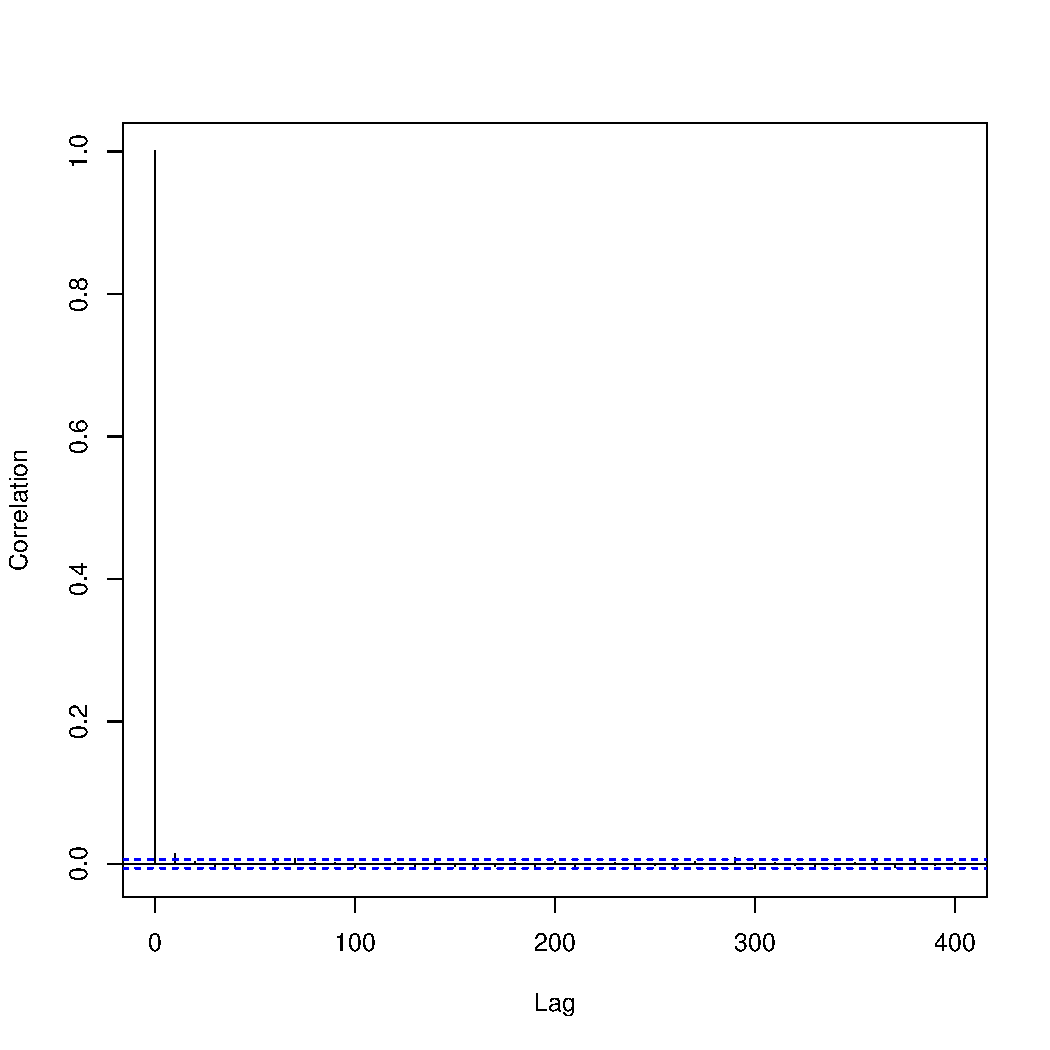
\includegraphics[scale = 0.45]{psi1acf.pdf}
\label{acf}}
\centering
\qquad
\centering
\subfloat[]
  {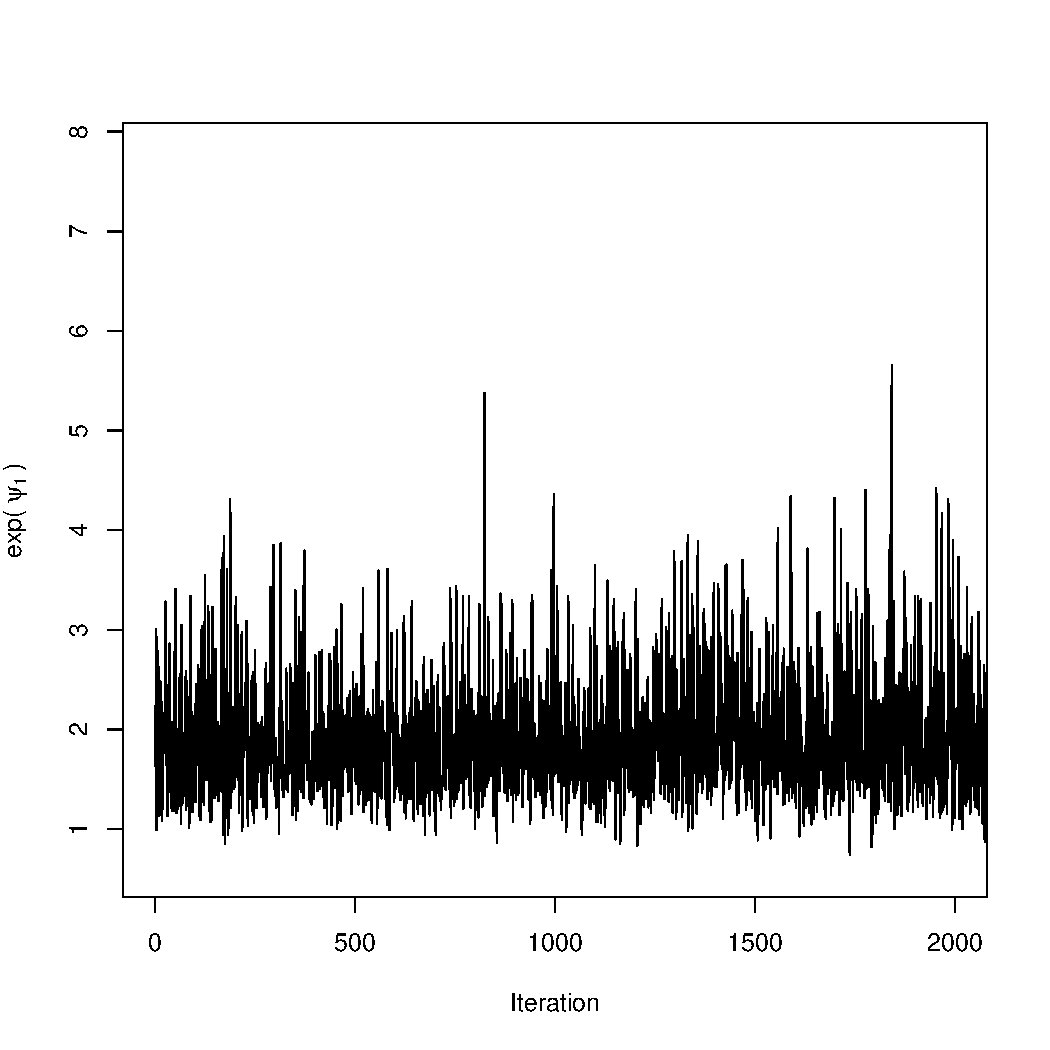
\includegraphics[scale = 0.45]{psi1trace.pdf}
\label{trace}}
\caption{Trace and Autocorrelation plots for the odds ratio}
\end{figure}
 
\pagebreak

\paragraph{Appendix 1: model.txt}
\begin{verbatim}
model {
for (i in 1:N) {
psihat[i]~dnorm(psi[i],1/(sigma[i])^2)
psi[i]~dnorm(mu,1/tau^2)
}
mu~dnorm(0,1/(1000*tau^2))
tau<-1/sqrt(gam)
gam ~ dgamma(0.1,0.1)
}
\end{verbatim}

\paragraph{Appendix 2: script.txt}
\begin{verbatim}
model clear
data clear
model in "model.txt"
data in "data.txt"
compile
inits in "initial_1.txt"
initialize
update 100000
monitor mu, thin(10)
monitor psi, thin(10)
monitor gam, thin(10)
update 1000000
coda *
\end{verbatim}

\paragraph{Appendix 3: R code}

\begin{verbatim}
library(coda)
res = read.coda("CODAchain1.txt", "CODAindex.txt")
psi1 = exp(res[,2])


pdf("psi1trace.pdf")
plot(as.numeric(psi1),  type= 'l',xlim = c(0,2000),
xlab = "Iteration", 
ylab = expression("exp(" ~ psi[1]~")")) ##trace plot
dev.off()

pdf("psi1acf.pdf")
acf(psi1, lag.max = 40, xlab = "Lag", 
ylab = "Correlation", main="")
## autocorrelation plot
dev.off()

pdf("psi1density.pdf")
plot(density(psi1),xlab = "x",ylab = "f(x)", 
main = expression("Density Plot for exp(" ~ psi[1]~")"))
dev.off()
prob = (1/length(psi1))*sum(psi1>1)
prob
\end{verbatim}
\end{document}